\frame{
  \begin{block}{Esempio Calcolo Performance}
    
    \begin{itemize}
      \item Eventi del log $(A, 1s), (B, 2s), (C, 4), (D, 8s)$ 
      \item Sequenza di transizioni del log replay  $A, B, C, t1, D$
      \item Risultato della sequenza \textquotedblleft eager\textquotedblright $A, B, t1, C, D$
    \end{itemize}

  \end{block}
  \begin{center}
    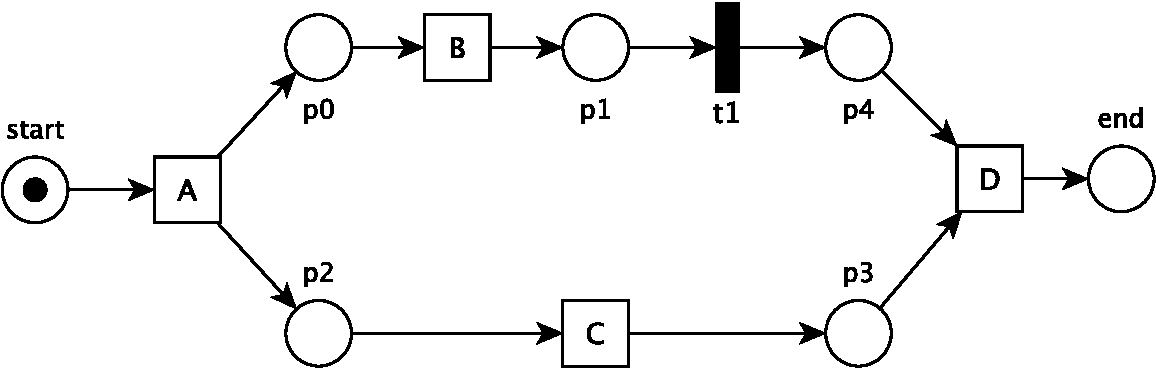
\includegraphics[scale=0.30]{./fig/LogReplay3a}
  \end{center}
  \begin {block}{Misure}
    \begin{tabular}{ccc}
                  \\
       $\TSync$   \\
       $\TTot$    \\
    \end{tabular}
  \end{block}
}

\frame{
  \begin{block}{Esempio Calcolo Performance}
    
    \begin{itemize}
      \item Eventi del log $\alert{(A, 1s)}, (B, 2s), (C, 4), (D, 8s)$ 
      \item Sequenza di transizioni del log replay  $A, B, C, t1, D$
      \item Risultato della sequenza \textquotedblleft eager\textquotedblright $\alert{A}, B, t1, C, D$
    \end{itemize}

  \end{block}
  \begin{center}
    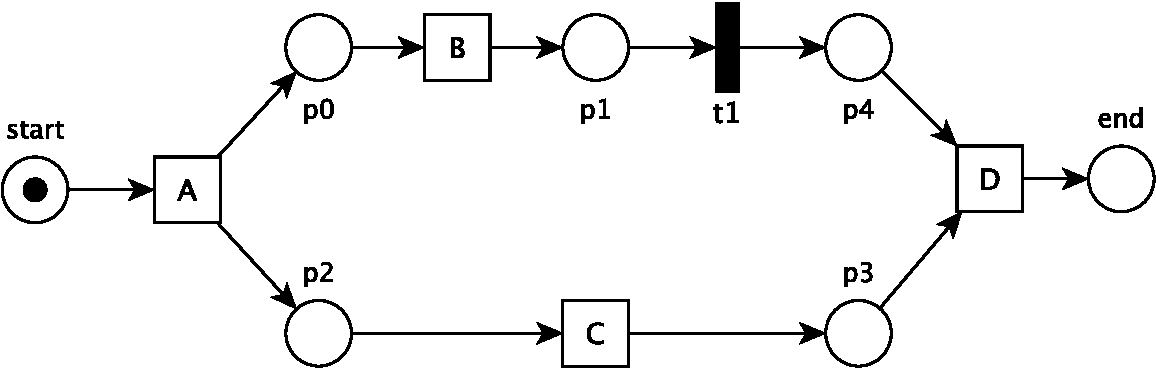
\includegraphics[scale=0.30]{./fig/LogReplay3a}
  \end{center}
  \begin {block}{Misure}
    \begin{tabular}{ccc}
                  \\
       $\TSync$   \\
       $\TTot$    \\
    \end{tabular}
  \end{block}
}

\frame{
  \begin{block}{Esempio Calcolo Performance}
    
    \begin{itemize}
      \item Eventi del log $\alert{(A, 1s)}, (B, 2s), (C, 4), (D, 8s)$ 
      \item Sequenza di transizioni del log replay  $A, B, C, t1, D$
      \item Risultato della sequenza \textquotedblleft eager\textquotedblright $\alert{A}, B, t1, C, D$
    \end{itemize}

  \end{block}
  \begin{center}
    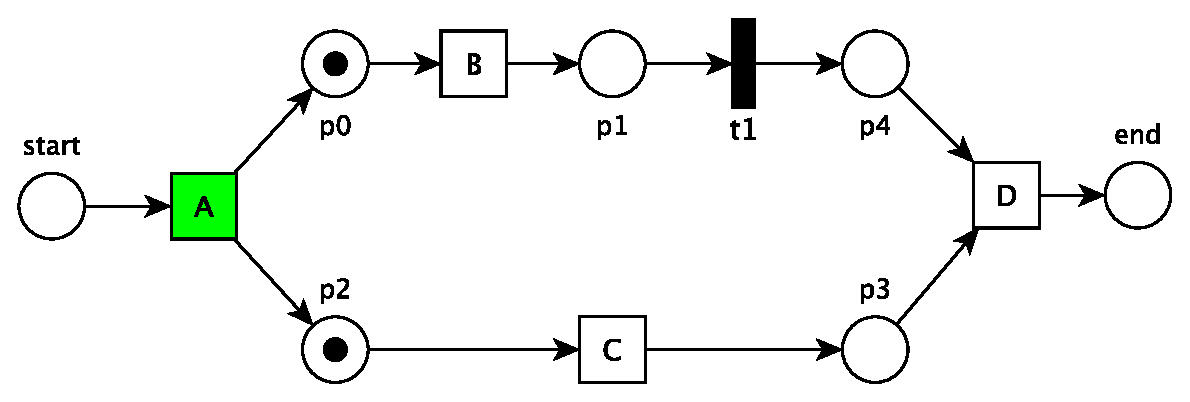
\includegraphics[scale=0.30]{./fig/LogReplay3b}
  \end{center}
  \begin {block}{Misure}
    \begin{tabular}{ccc}
                  & p0 & p2 \\
       $\TSync$   & 0  & 0  \\
       $\TTot$    &    &    \\
    \end{tabular}
  \end{block}
}
\frame{
  \begin{block}{Esempio Calcolo Performance}
    
    \begin{itemize}
      \item Eventi del log $(A, 1s), \alert{(B, 2s)}, (C, 4), (D, 8s)$ 
      \item Sequenza di transizioni del log replay  $A, B, C, t1, D$
      \item Risultato della sequenza \textquotedblleft eager\textquotedblright $A, \alert{B}, t1, C, D$
    \end{itemize}

  \end{block}
  \begin{center}
    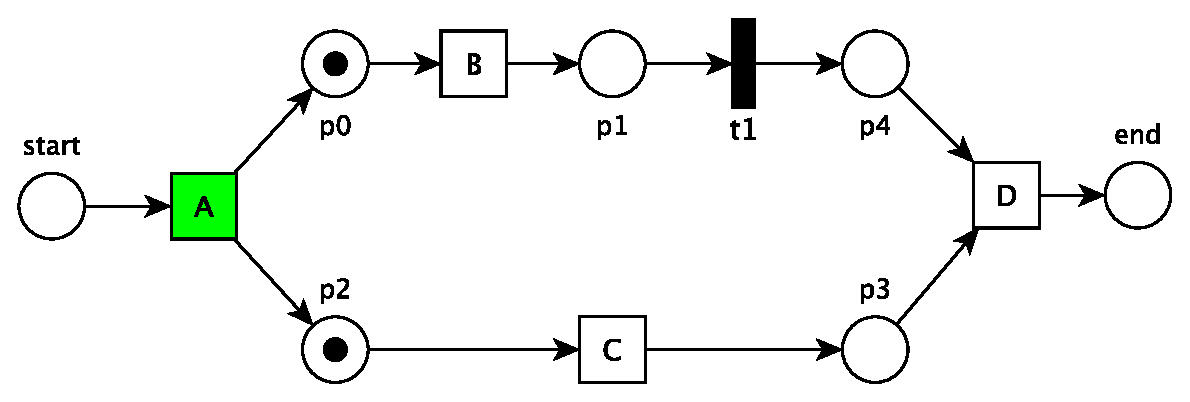
\includegraphics[scale=0.30]{./fig/LogReplay3b}
  \end{center}
  \begin {block}{Misure}
    \begin{tabular}{ccc}
                  & p0 & p2 \\
       $\TSync$   & 0  & 0  \\
       $\TTot$    &    &    \\
    \end{tabular}
  \end{block}
}
\frame{
  \begin{block}{Esempio Calcolo Performance}
    
    \begin{itemize}
      \item Eventi del log $(A, 1s), \alert{(B, 2s)}, (C, 4), (D, 8s)$ 
      \item Sequenza di transizioni del log replay  $A, B, C, t1, D$
      \item Risultato della sequenza \textquotedblleft eager\textquotedblright $A, \alert{B}, t1, C, D$
    \end{itemize}

  \end{block}
  \begin{center}
    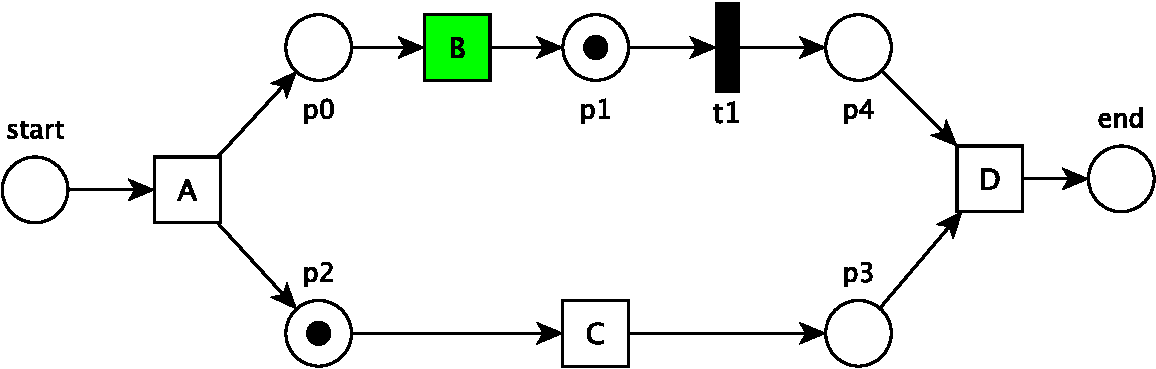
\includegraphics[scale=0.30]{./fig/LogReplay3c}
  \end{center}
  \begin {block}{Misure}
    \begin{tabular}{cccccc}
                  & p0 & p2 & p1 \\
       $\TSync$   & 0  & 0  & 0  \\
       $\TTot$    & 1  &    &    \\
    \end{tabular}
  \end{block}
}

% Attivazione di t1
\frame{
  \begin{block}{Esempio Calcolo Performance}
    
    \begin{itemize}
      \item Eventi del log $(A, 1s), \alert{(B, 2s)}, (C, 4), (D, 8s)$ 
      \item Sequenza di transizioni del log replay  $A, B, C, t1, D$
      \item Risultato della sequenza \textquotedblleft eager\textquotedblright $A, B, \alert{t1}, C, D$
    \end{itemize}

  \end{block}
  \begin{center}
    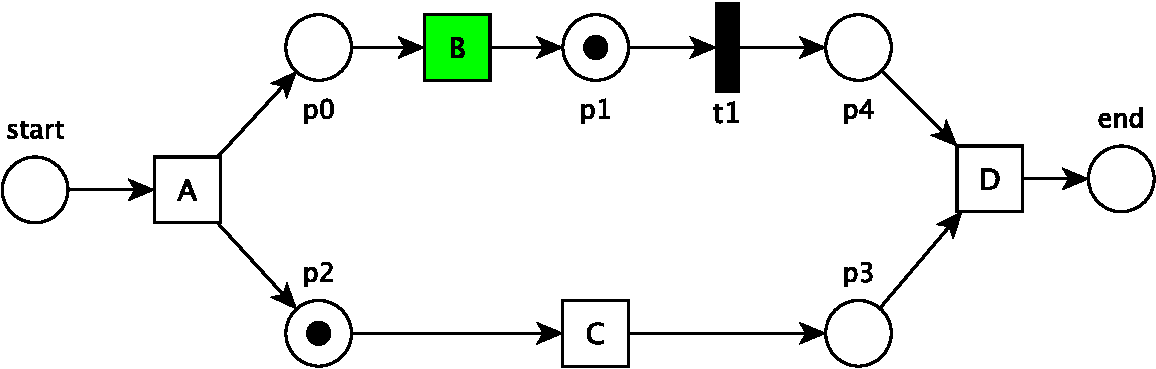
\includegraphics[scale=0.30]{./fig/LogReplay3c}
  \end{center}
  \begin {block}{Misure}
    \begin{tabular}{cccccc}
                  & p0 & p2 & p1 \\
       $\TSync$   & 0  & 0  & 0  \\
       $\TTot$    & 1  &    &    \\
    \end{tabular}
  \end{block}
}
\frame{
  \begin{block}{Esempio Calcolo Performance}
    
    \begin{itemize}
      \item Eventi del log $(A, 1s), \alert{(B, 2s)}, (C, 4), (D, 8s)$ 
      \item Sequenza di transizioni del log replay  $A, B, C, t1, D$
      \item Risultato della sequenza \textquotedblleft eager\textquotedblright $A, B, \alert{t1}, C, D$
    \end{itemize}
  \end {block}
  \begin{center}
    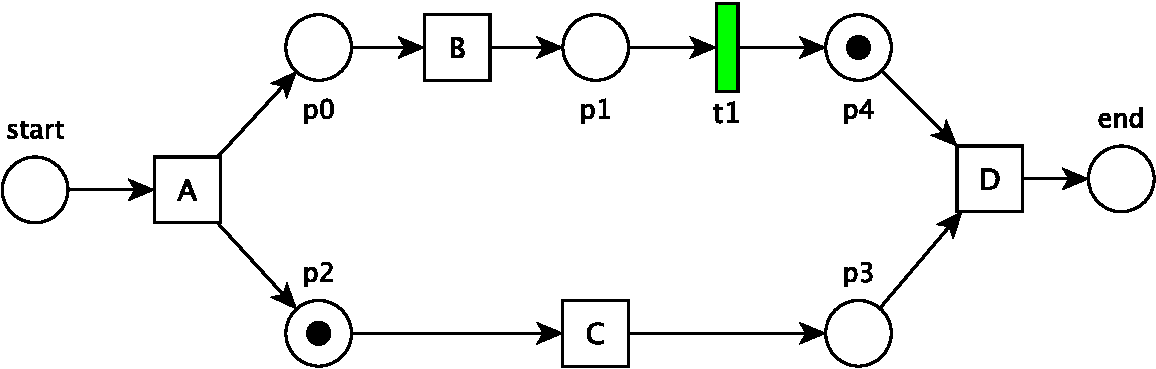
\includegraphics[scale=0.30]{./fig/LogReplay4d}
  \end{center}
  \begin {block}{Misure}
    \begin{tabular}{cccccc}
                  & p0 & p2 & p1 & p3 & p4 \\
       $\TSync$   & 0  & 0  & 0  &    &    \\
       $\TTot$    & 1  &    & 0  &    &    \\
    \end{tabular}
  \end{block}
}

\frame{
  \begin{block}{Esempio Calcolo Performance}
    
    \begin{itemize}
      \item Eventi del log $(A, 1s), (B, 2s), \alert{(C, 4)}, (D, 8s)$ 
      \item Sequenza di transizioni del log replay  $A, B, C, t1, D$
      \item Risultato della sequenza \textquotedblleft eager\textquotedblright $A, B, t1, \alert{C}, D$
    \end{itemize}
  \end {block}
  \begin{center}
    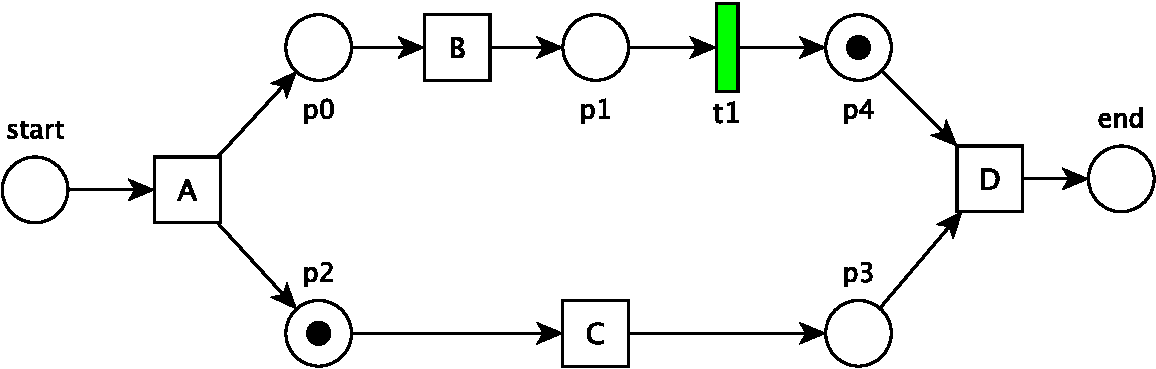
\includegraphics[scale=0.30]{./fig/LogReplay4d}
  \end{center}
  \begin {block}{Misure}
    \begin{tabular}{cccccc}
                  & p0 & p2 & p1 & p3 & p4 \\
       $\TSync$   & 0  & 0  & 0  &    &    \\
       $\TTot$    & 1  &    & 0  &    &    \\
    \end{tabular}
  \end{block}
}
\frame{
  \begin{block}{Esempio Calcolo Performance}
    
    \begin{itemize}
      \item Eventi del log $(A, 1s), (B, 2s), \alert{(C, 4)}, (D, 8s)$ 
      \item Sequenza di transizioni del log replay  $A, B, C, t1, D$
      \item Risultato della sequenza \textquotedblleft eager\textquotedblright $A, B, t1, \alert{C}, D$
    \end{itemize}
  \end {block}
  \begin{center}
    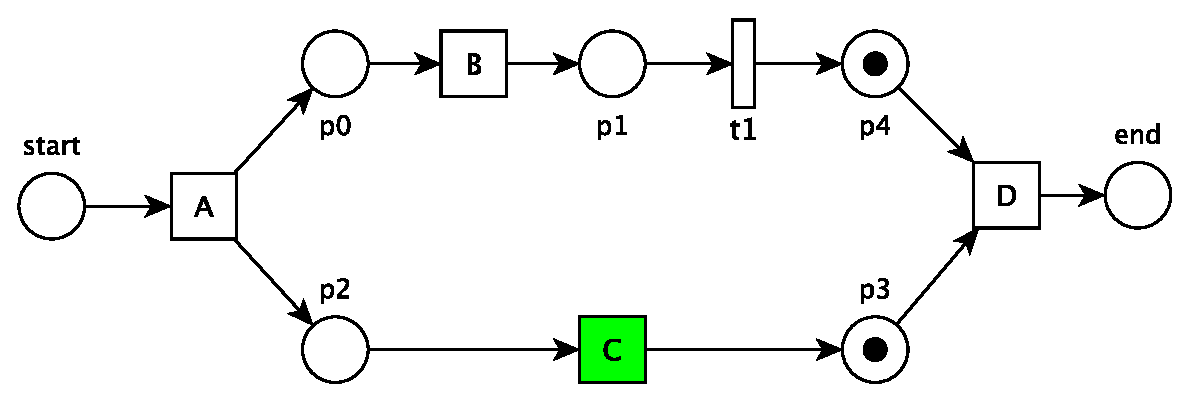
\includegraphics[scale=0.30]{./fig/LogReplay4e}
  \end{center}
  \begin {block}{Misure}
    \begin{tabular}{cccccc}
                  & p0 & p2 & p1 & p3 & p4 \\
       $\TSync$   & 0  & 0  & 0  & 0  & 2  \\
       $\TTot$    & 1  & 2  & 0  &    &    \\
    \end{tabular}
  \end{block}
}
\frame{
  \begin{block}{Esempio Calcolo Performance}
    
    \begin{itemize}
      \item Eventi del log $(A, 1s), (B, 2s), (C, 4), \alert{(D, 8s)}$ 
      \item Sequenza di transizioni del log replay  $A, B, C, t1, D$
      \item Risultato della sequenza \textquotedblleft eager\textquotedblright $A, B, t1, C, \alert{D}$
    \end{itemize}
  \end {block}
  \begin{center}
    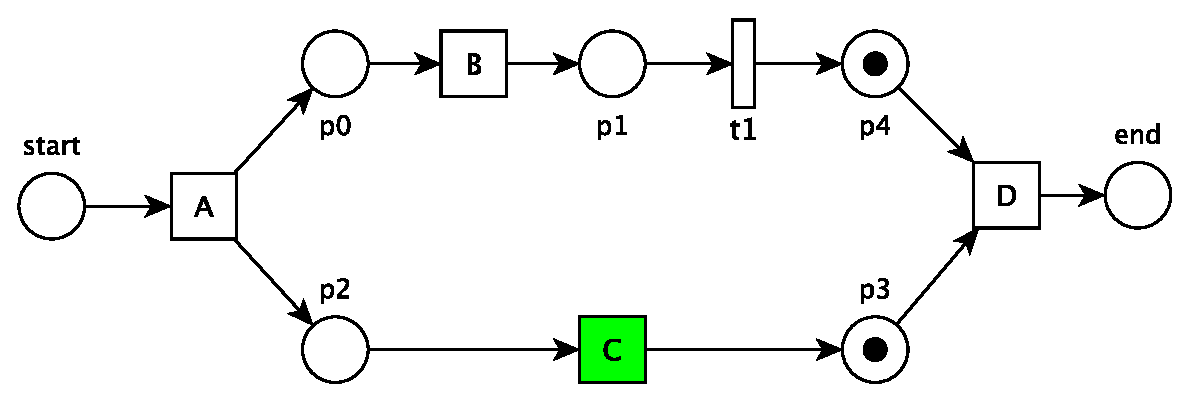
\includegraphics[scale=0.30]{./fig/LogReplay4e}
  \end{center}
  \begin {block}{Misure}
    \begin{tabular}{cccccc}
                  & p0 & p2 & p1 & p3 & p4 \\
       $\TSync$   & 0  & 0  & 0  & 0  & 2  \\
       $\TTot$    & 1  & 2  & 0  &   &   \\
    \end{tabular}
  \end{block}
}
\frame{
  \begin{block}{Esempio Calcolo Performance}
    
    \begin{itemize}
      \item Eventi del log $(A, 1s), (B, 2s), (C, 4), \alert{(D, 8s)}$ 
      \item Sequenza di transizioni del log replay  $A, B, C, t1, D$
      \item Risultato della sequenza \textquotedblleft eager\textquotedblright $A, B, t1, C, \alert{D}$
    \end{itemize}
  \end {block}
  \begin{center}
    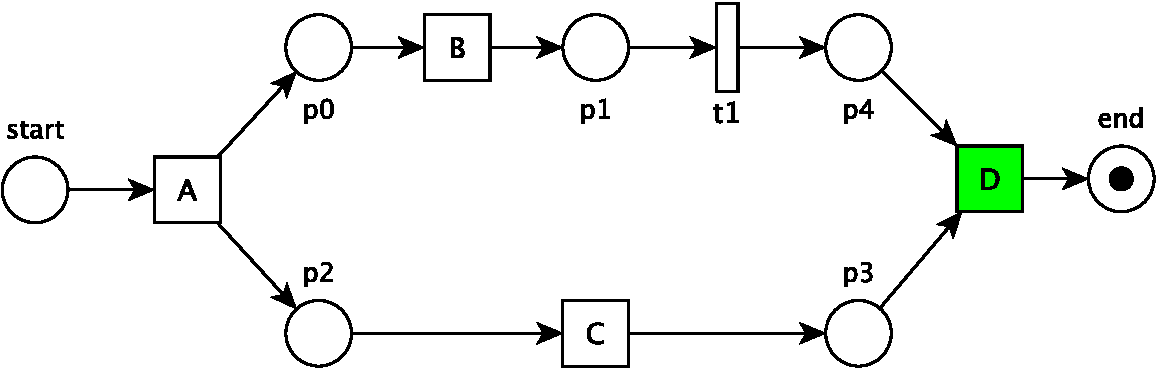
\includegraphics[scale=0.30]{./fig/LogReplay4f}
  \end{center}
  \begin {block}{Misure}
    \begin{tabular}{cccccc}
                  & p0 & p2 & p1 & p3 & p4 \\
       $\TSync$   & 0  & 0  & 0  & 0  & 2  \\
       $\TTot$    & 1  & 2  & 0  & 4  & 6  \\
    \end{tabular}
  \end{block}
}
%%% Local Variables: 
%%% mode: latex
%%% TeX-master: "main"
%%% End: 
